\ifx\wholebook\relax\else
\input{../Common.tex}
\input{../macroes.tex}
\begin{document}
\fi
\chapter{Conditional Loops}\label{ch:ConditionalLoops}

@@dank: I've finally figured out a problem that has been nagging at me for a while: the term 'message', which got a specific definition in Chapter 4, is frequently used for the concept 'expression' or 'statement'.  This reduces the clarity of the text.  I'll start suggesting changes where I notice the misuse. @@
\replace{Having conditions is a}{Conditions are} good \replace{tool}{tools} for expressing complex programs. However, conditions are not enough. \replace{Sometimes we would like}{Some programs need} to combine loops and conditions. \replace{In fact we would like}{Loops and conditions are combined in} \replace{conditional loops}{\emph{conditional loops} \index{conditional loops}}, \replace{\ie\}{i.e.} loops that repeat \replace{sequence of messages}{a block of expressions} while a certain condition holds. \replace{In this}{This} chapter \replace{we present}{presents} the conditional loops offered by \st using simple examples. \add{\paragraph
}
@@dank: The next paragraph is a forward reference --- I recommend moving it to the end of the chapter or omitting it completely.@@ 
\replace{We}{The book following this one} will use \remove{a lot} conditional loops \add{a lot,} to simulate animal behavior  and  to define strategies \replace{to escape maze or following paths \book}{for escaping a maze or following a path}.

\section{Conditional Loops}
@@dank: As I suggested in the previous chapter, I think 'block' would be a better name than 'messages' or 'sequence of messages'. This time I'll be bolder and make the substitution without waiting for your response. @@
The idea behind conditional loops is that a \replace{sequence of messages}{block of expressions} is repeated \replace{while}{as long as} a certain condition holds. \st defines two messages\add{,} \index{whileTrue:}\ct{whileTrue:} and \index{whileFalse:}\ct{whileFalse:}\add{,} that allow you to define conditional loops\remove{ as shown  below}. @@dank: I recommend deleting the next sentence as redundant with the following paragraph, but if you want to keep it, change it to: \replace{Let us}{Let's} start \replace{by}{with} an example.@@

\paragraph{An Example.} \replace{Let us}{Let's} take a simple example to illustrate their use.  Imagine we want a robot to move \remove{in the direction of the} north until its y coordinate is smaller than 100 pixels.  A solution using a conditional loop is shown by \tmthref{mth:upto}\replace{ and that}{; it} can be invoked as shown in \tscrref{scr:upto}.

@@dank: I recommend reordering these, so they appear in the same order as the references in the previous paragraph (the method before the script). It would reduce the reader's effort and the chances of mistaking one for the other.  Also would 'northPast100' (or 'upPast100') be a better method name? @@
\begin{scriptwithtitle}{Invoking \ct{upTo100}}\label{scr:upto}
| \caro |
\caro := \Turtle new.
\caro upTo100
\end{scriptwithtitle}

\begin{method}\label{mth:upto}
upTo100
   "\replace{Make forward}{Move} the receiver \add{north} until its \replace{ordinates}{ordinate} is smaller than 100"
   self north.
   \textbf{[self center y \replace{>}{>=} 100]}
      whileTrue: \textbf{[self go: 10].}
   self color: Color green.
\end{method}

\replace{Let us carefully}{Let's} look \add{carefully} at \replace{what's happen}{what happens} when this method is executed. 
\begin{enumerate}
\item The expression \ct{self north} is not part of the conditional loop, \replace{therefore}{so} it is executed once. 

\item \replace{Then the}{The} condition\add{,} which is expressed as a block\replace{ \ct{[self center y > 100]}}{,} is executed.  \add{In this example the condition is \ct{[self center y >= 100]}.}


\item \ct{whileTrue:}, the \replace{conditional loop}{method} name,  defines the meaning of the loop:  when the result of the condition is true\replace{ and only then}{,} the conditional \replace{messages}{block} specified as argument of the method \ct{whileTrue:}\replace{,  \ct{[self go: 10]}, are}{ is} executed. \add{In the example, this step executes the block \ct{[self go: 10]} if the condition \ct{[self center y >= 100]} is true.} Once the execution of the conditional \replace{messages terminates}{block finishes,} the process restarts \replace{as in point}{at step} 2.

\item When the result of the condition \ct{[self center y \replace{>}{>=} 100]} \add{in step 2} is false, the conditional \replace{messages are}{block is} \textit{not} executed and the loop stops. \add{The program goes on to step 5. \paragraph

\item} The \replace{messages}{expressions} following the conditional expression are executed\replace{: here}{.  In the example,} the expression \ct{self color: Color green} gets executed and the method terminates. 
\end{enumerate}

\replace{As we already mentioned it the}{The} meaning of the loop is defined by its \add{method} name: \ct{whileTrue:} executes the condition\add{,} and \add{when the condition is true, also} executes the conditional \replace{messages when the condition is true}{block}.  \ct{whileFalse:} \replace{does the same}{is similar} but executes the conditional \replace{message}{block} only when the conditional is false. \add{As before, the conditional block can contain a single statement or a series of statements. \paragraph
}
Figure~\ref{fig:conditionalLoopsPicturehere}
shows that a conditional \replace{loops}{loop} is composed of  a \emph{condition} and \add{a} \emph{conditional \replace{messages}{block}}. 

\begin{figure}[h]
\begin{center}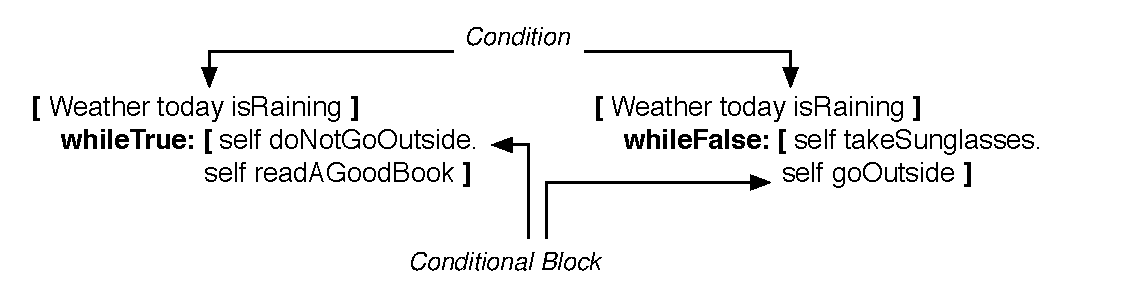
\includegraphics{conditionalLoopsPicture}
\caption{\replace{The}{A} \ct{whileTrue:} conditional \replace{loops}{loop} is composed of a condition and a \remove{sequence of} conditional \replace{messages}{block}.\label{fig:conditionalLoopsPicturehere}}
\end{center}
\end{figure}

\fprod{the following should be in a frame}
\index{whileTrue:}\ct{whileTrue:} and \index{whileFalse:}\ct{whileFalse:} allow you to define conditional loops\replace{ \ie}{, i.e.} the conditional \replace{messages are}{block is} repeated while the condition holds. \\
\begin{nalltt}
\textbf{[} condition \textbf{] whileFalse:}
  \textbf{[} conditional \replace{messages}{block} \textbf{]}

\textbf{[} condition \textbf{] whileTrue:}
  \textbf{[} conditional \replace{messages}{block} \textbf{]}
\end{nalltt}
\fprod{until here}

\replace{As for}{Like} \ct{ifTrue:} and \ct{ifFalse:}, \ct{whileTrue:} can be \replace{substitued by}{converted to} \ct{whileFalse:} by negating \add{(logically reversing)} the condition.  Use \replace{the}{whichever} method \remove{that} helps you \remove{to} understand \remove{the best} your program\add{ better}. \add{\paragraph
}
Try to \replace{express the}{define a} method \add{like} \ct{upTo100} \replace{but using the method}{that uses} \ct{whileFalse:}\add{ instead of \ct{whileTrue:}}. \replace{Try to make}{Then define a method that makes} the robot \replace{moving}{move} one pixel \replace{by one pixel}{at a time, instead of 10 pixels in each step.} \replace{and compare}{Compare} the exact position where it stops.

\subsection*{}
Sometimes defining correct conditional loops is difficult. \replace{Indeed it}{It} is easy to forget to check \remove{carefully} the condition \add{carefully,} and the loop can \add{repeat} endlessly\remove{ loop}. While writing a conditional loop you should always keep in mind that the loop should somehow tend toward the end of the loop\replace{ \ie\}{, i.e.} tend toward a situation that makes the condition not hold anymore. 

\replace{Perform the following experience}{Try this experiment}: move the robot by using the black halo close to the top edge of the window, \replace{\ie\}{ i.e.} be sure its y coordinate is smaller than 100. Then invoke the method \ct{upTo100}\replace{, as you should}{.  As you} see\add{,} nothing happens. This is \replace{normal,}{as expected:} the method is invoked and the expression \ct{self center y \replace{>}{>=} 100} is false\replace{ as}{, because} the \add{vertical} position of the robot is smaller than 100. Therefore the conditional \replace{messages are}{block is} not executed. 


\section{Stopping an \replace{Infinitie}{Infinite} Loop}
It is not exceptional to write \add{an} endless loop. \replace{Practically}{For \ct{whileFalse:}}, this happens because the \replace{boolean expression}{condition} never returns true\replace{ for \ct{whileFalse:} and}{; for \ct{whileTrue:}, it's because the condition never returns} false\remove{ for \ct{whileTrue:}}. \add{\paragraph
} 
\replace{You}{If you do write an endless loop, you} can stop \index{stopping an endless loop} \replace{a loop}{it} by pressing \add{the interrupt key combination.  It is} Apple-. on Mac or Alt . or Control-C on other platforms. Then to understand why the loop \replace{does}{did} not terminate\add{,} you can use the debugger \remove{that pops up} by clicking \replace{its}{the} Debug button\add{ when the error message pops up}.

\replace{In fact a}{A} conditional loop can \add{repeat} endlessly \remove{loop} when the conditional \replace{messages do not}{block doesn't} perform an action that \replace{tends towards a state that breaks}{will eventually break} the condition\replace{ \ie make}{, i.e. stop} the condition \replace{not}{from} holding anymore. \replace{Let us illustrate}{\paragraph

Let's consider} this difficult point in the case of our example.  \replace{We see that the}{The} distance between the robot and the \replace{vertical point having 100 as}{horizontal line with the} y value \add{of 100} gets smaller and smaller. \replace{In the example, to}{To} be sure that the loop \replace{gets}{has} a chance to terminate,  the conditional \replace{messages}{block} should somehow reduce this distance.  @@dank: I think the logic of the previous paragraph would be easier to follow if the last two sentences were rearranged, so the solution followed the requirement; something like "As long as the robot center's y coordinate is too big (\ct{>= 100}), the loop will continue. So to be sure that the loop will terminate, the conditional block must somehow reduce the robot's y coordinate.  The expression \ct{self go: 10} in the conditional block does this, because the y coordinate gets smaller as the robot moves north."@@    

\replace{Let us}{Let's} look at a trivial case \add{of an infinite loop,} shown in the method \ct{upTo100Infinite} (\ref{mth:uptoinfinite}). \replace{Even if this may looks obvious,}{This may seem obvious:} the method~\ref{mth:uptoinfinite} cannot terminate because  the conditional \replace{messages}{block} cannot change the condition. Here, the conditional \replace{messages increase}{block increases}  the value of the y \replace{coordinates, therefore}{coordinate, so} the chance that the condition may evaluate to false reduces \add{on} each \replace{turn}{repetition}. This example is exaggerated but it illustrates clearly the problem of specifying 
loops that \replace{terminates}{terminate}. 

\begin{method}\label{mth:uptoinfinite}
@@dank: would 'southPast100' (or 'downPast100') be a better name?  It isn't always infinite.@@
upTo100Infinite
   "\replace{Make forward}{Move} the receiver \add{south} until its \replace{ordinates}{ordinate} is smaller than 100"
   \textbf{self south.}
   \textbf{[self center y \replace{>}{>=} 100]}
      whileTrue: \textbf{[self go: 10].}
   self color: Color green
\end{method}
@@dank: This is an example of why I want a copy of the student's image.  In my mock-up (based on StarSqueakMorph and StarSqueakTurtle), this loop does terminate because the bot wraps around to the top of the window when it crosses the lower boundary.@@

\largecadre{When you are defining a loop always ask yourself if there is a possibility that the condition \replace{is not}{might never be} met. This seems obvious but if the condition does not have a chance to \replace{be false}{fail,} the loop will never finish.}

\section{@@@Using the debugger@@@}
@@dank: This section is present in my copy of BookBasicLevel.pdf. @@


\section{Deeper into \ct{whileTrue:} and \ct{whileFalse:}}
The condition of a conditional loop does not have to \remove{only} contain \add{just} a \replace{boolean}{single} expression. It \add{is a block that} can contain a sequence of \replace{messages}{expressions,} as \replace{soon}{long} as the last \replace{conditional message}{expression in the condition} returns \replace{a boolean as shown by the following template}{either true or false}. This allows one to express \replace{different conditional loops}{more complicated conditions}. @@dank: I recommend omitting the next sentence as unhelpful and a distraction.@@ \remove{Note that other programming languages do not allow this, but provide different conditional loops.}

\add{Here is an example of a condition with more than one expression.}
\begin{template}
\textbf{[}self doThis.
anObject doThat.
\emph{self isStillWorking}\textbf{] whileTrue: 
   [}self grumbleAndKeepOnWorking\textbf{]}
\end{template}

Therefore \replace{we can}{you could} change the method \ct{upTo100} to \remove{be as} the method~\ref{mth:notTheSame}. \replace{As its name tells us, while}{While}
this method \replace{looks}{seems} nearly the same as \remove{the} \ct{upTo100}, it \replace{is}{sometimes has a} different \add{effect}. Try to understand \replace{where is}{what} the difference\add{ is}. For example, add a trace or invoke the debugger in \tmthref{mth:notTheSame} and analyze it. 

\begin{method}\label{mth:notTheSame}
@@dank: would differentNorthPast100 be a better name?@@
notTheSameUpTo100
   "\replace{Make forward}{Move} the receiver \add{north} until its \replace{ordinates}{ordinate} is smaller than 100"
   self north.
   [self go: 10.
   self center y \replace{>}{>=} 100]
      whileTrue: [ ].
   self color: Color green
\end{method}

As the condition is \add{always executed} at least \remove{executed} once, the main difference is that the robot will move even if it \remove{is} already  \replace{at position}{has a y coordinate} smaller than 100.  

\section{About the Use of \ct{[]}}\label{sec:useOfparent}
You may have difficulties \replace{to remember when}{remembering whether} to \replace{put}{use} squared brackets \ct{[]} \replace{and}{or} not. 
There are basically two rules in \sq. You surround an expression \add{(or group of expressions)} with \ct{[} and \ct{]} when:  

\begin{itemize}
\item You need to execute \remove{several times} the same expression \add{(or group of expressions) several times}. For example, 
\begin{itemize}
\item \ct{4 timesRepeat: [\caro go: 10; turnLeft:90]} repeats \remove{4 times} the \replace{messages}{expression} \ct{\caro go: 10; turnLeft:90}\replace{,}{ 4 times.}

\item \ct{1 to: 10 do: [:i | Transcript show: i printString ; cr]} repeats \remove{ten times} the 
\add{block} \ct{[:i | Transcript show: i printString ; cr]} \replace{which}{ten times.  Each time it} prints the number to the transcript. 
@@dank: I suggest avoiding examples that use unfamiliar concepts or constructs, other than the one it is designed to illustrate.  The previous example includes an interval, do:, and a block argument, which haven't been introduced in this book.  I recommend substituting an example which uses only familiar constructs.@@
\end{itemize}

\item The expression \add{(or group of expressions)} is not always executed. 
@@dank: Would it be more accurate to say "The expression is executed a variable number of times"?For instance the second example doesn't illustrate the original rule, because the condition [self center y \replace{>}{>=} 100] is always executed at least once. This will confuse readers with logical minds.  I recommend rewriting the rule or the example. @@
For example,

\begin{itemize} 
\item \ct{dist < 200 ifTrue: [self color: Color red]} only executes \ct{self color: Color red} under certain circumstances\replace{,}{.} 
 
\item \ct{[self center y > 100] whileTrue: [self go: 10]} repeats \remove{multiple times conditionally} both \ct{self center y > 100} and \ct{self go: 10}\replace{, therefore}{multiple times, depending on conditions.  Therefore} the receiver and the argument are blocks.
\end{itemize}
@@dank: Unfortunately these rules aren't completely accurate; for instance 1 timesRepeat: and 0 timesRepeat: still require block arguments.  I think more accurate rules (for constructs introduced so far) can be stated almost as simply: "The argument of a conditional message (ifTrue:, ifFalse:, ifTrue:ifFalse:) or conditional loop message (whileTrue:, whileFalse:) is enclosed in square brackets. The receiver of a conditional loop message (whileTrue:, whileFalse:) is enclosed in square brackets."  I suggest you include a statement of the real rules as well. @@
\end{itemize}

@@dank: My version of BookBasicLevel.pdf has a section 'A Simple Application' in this chapter that is missing from ConditionalLoops.tex.@@

\section{Summary}

\begin{table}[h]
\small
\centering
\begin{tabular}{||p{5cm}|p{10cm}||} \hline
Method&Description\\ \hline
\begin{nalltt}
\textbf{[}aCondition\textbf{] whileFalse:}
  \textbf{[}\replace{SequenceOfMessages}{SequenceOfExpressions} \textbf{]}
\end{nalltt}
&Execute \ct{aCondition}\add{;}  if it is false\replace{ executes}{, execute} \ct{\replace{SequenceOfMessages}{SequenceOfExpressions}} and \replace{repeats}{repeat} this step\replace{, if}{. If} \ct{aCondition} is true, \replace{passes}{pass} to the next expression without executing  \ct{\replace{SequenceOfMessages}{SequenceOfExpressions}}. \\  \hline

\begin{nalltt}
\textbf{[} aCondition \textbf{] whileTrue:}
  \textbf{[}\replace{SequenceOfMessages}{SequenceOfExpressions} \textbf{]}
\end{nalltt} 
&Execute \ct{aCondition}\add{;}  if it is true\add{,} execute \ct{\replace{SequenceOfMessages}{SequenceOfExpressions}} and \replace{repeats}{repeat} this step\replace{, if}{. If} \ct{aCondition} is false, \replace{passes}{pass} to the next expression without executing  \ct{\replace{SequenceOfMessages}{SequenceOfExpressions}}. \\  \hline\\ \remove{\hline}
\end{tabular}
\end{table}



\ifx\wholebook\relax\else\end{document}\fi





